\documentclass[journal]{vgtc}                % final (journal style)
%\documentclass[review,journal]{vgtc}         % review (journal style)
%\documentclass[widereview]{vgtc}             % wide-spaced review
%\documentclass[preprint,journal]{vgtc}       % preprint (journal style)

%% Uncomment one of the lines above depending on where your paper is
%% in the conference process. ``review'' and ``widereview'' are for review
%% submission, ``preprint'' is for pre-publication, and the final version
%% doesn't use a specific qualifier.

%% Please use one of the ``review'' options in combination with the
%% assigned online id (see below) ONLY if your paper uses a double blind
%% review process. Some conferences, like IEEE Vis and InfoVis, have NOT
%% in the past.

%% Please note that the use of figures other than the optional teaser is not permitted on the first page
%% of the journal version.  Figures should begin on the second page and be
%% in CMYK or Grey scale format, otherwise, colour shifting may occur
%% during the printing process.  Papers submitted with figures other than the optional teaser on the
%% first page will be refused. Also, the teaser figure should only have the
%% width of the abstract as the template enforces it.

%% These few lines make a distinction between latex and pdflatex calls and they
%% bring in essential packages for graphics and font handling.
%% Note that due to the \DeclareGraphicsExtensions{} call it is no longer necessary
%% to provide the the path and extension of a graphics file:
%% 
\includegraphics{diamondrule} is completely sufficient.
%%
\ifpdf%                                % if we use pdflatex
  \pdfoutput=1\relax                   % create PDFs from pdfLaTeX
  \pdfcompresslevel=9                  % PDF Compression
  \pdfoptionpdfminorversion=7          % create PDF 1.7
  \ExecuteOptions{pdftex}
  \usepackage{graphicx}                % allow us to embed graphics files
  \DeclareGraphicsExtensions{.pdf,.png,.jpg,.jpeg} % for pdflatex we expect .pdf, .png, or .jpg files
\else%                                 % else we use pure latex
  \ExecuteOptions{dvips}
  \usepackage{graphicx}                % allow us to embed graphics files
  \DeclareGraphicsExtensions{.eps}     % for pure latex we expect eps files
\fi%

%% it is recomended to use ``\autoref{sec:bla}'' instead of ``Fig.~\ref{sec:bla}''
\graphicspath{{figures/}{pictures/}{images/}{./}} % where to search for the images

\usepackage{microtype}                 % use micro-typography (slightly more compact, better to read)
\PassOptionsToPackage{warn}{textcomp}  % to address font issues with \textrightarrow
\usepackage{textcomp}                  % use better special symbols
\usepackage{mathptmx}                  % use matching math font
\usepackage{times}                     % we use Times as the main font
\renewcommand*\ttdefault{txtt}         % a nicer typewriter font
\usepackage{cite}                      % needed to automatically sort the references
\usepackage{tabu}                      % only used for the table example
\usepackage{booktabs}                  % only used for the table example
%% We encourage the use of mathptmx for consistent usage of times font
%% throughout the proceedings. However, if you encounter conflicts
%% with other math-related packages, you may want to disable it.

%% In preprint mode you may define your own headline.
%\preprinttext{To appear in IEEE Transactions on Visualization and Computer Graphics.}

%% If you are submitting a paper to a conference for review with a double
%% blind reviewing process, please replace the value ``0'' below with your
%% OnlineID. Otherwise, you may safely leave it at ``0''.
\onlineid{0}

%% declare the category of your paper, only shown in review mode
\vgtccategory{Research}
%% please declare the paper type of your paper to help reviewers, only shown in review mode
%% choices:
%% * algorithm/technique
%% * application/design study
%% * evaluation
%% * system
%% * theory/model
\vgtcpapertype{please specify}

%% Paper title.
\title{Assignment 2 - CS 458}

%% This is how authors are specified in the journal style

%% indicate IEEE Member or Student Member in form indicated below
\author{Amber Horvath, Alannah Oleson, and Katherine Bajno}
\authorfooter{
%% insert punctuation at end of each item
\item
 Amber Horvath, computer science student at Oregon State University: E-mail: horvatha@oregonstate.edu.
\item
 Alannah Oleson, computer science student at Oregon State University. E-mail: olesona@oregonstate.edu.
\item
 Katherine Bajno, computer science student at Oregon State University. E-mail: kbajno@oregonstate.edu
}

%other entries to be set up for journal
%\shortauthortitle{Firstauthor \MakeLowercase{\textit{et al.}}: Paper Title}

%% Abstract section.
\abstract {
On a large scale, many recent studies link high air pollution levels to the larger problem of climate
change. On a somewhat smaller scale, a large amount of air pollution can not only affect the climate
of a certain geographic region - it can also negatively affect the quality of life for those who
live there. Over time, the rate at which the air quality of a region is increasing or decreasing
can single the area out for inspection by climate scientists or give the inhabitants of the area
an indicator of the overall healthiness of the environment there.

To address both issues in a way that the average person can understand, we created a 
visualization of air pollution levels in the western United States. We use a treemap format
to represent the magnitude of 11 states' air pollution levels over the span of ten years. 
We also make use of a color gradient to indicate the rate at which polltion levels are increasing
or decreasing. This is a novel representation because much of this kind of data is presented in 
tables that are rather hard to parse. Our visualization, on the other hand, gives the user a good 
overview of general trends in the region at a glance, while still allowing them to drill down into
the details if they want to. This can benefit both average people (for instance, someone looking at
which state in the region they want to move to) and those with specialized needs such as climate
scientists.
}
% end of abstract

%% Keywords that describe your work. Will show as 'Index Terms' in journal
%% please capitalize first letter and insert punctuation after last keyword
%\keywords{Radiosity, global illumination, constant time}

%% ACM Computing Classification System (CCS). 
%% See <http://www.acm.org/class/1998/> for details.
%% The ``\CCScat'' command takes four arguments.



%% Uncomment below to include a teaser figure.


%% Uncomment below to disable the manuscript note
\renewcommand{\manuscriptnotetxt}{}

%% Copyright space is enabled by default as required by guidelines.
%% It is disabled by the 'review' option or via the following command:
% \nocopyrightspace

\vgtcinsertpkg

%%%%%%%%%%%%%%%%%%%%%%%%%%%%%%%%%%%%%%%%%%%%%%%%%%%%%%%%%%%%%%%%
%%%%%%%%%%%%%%%%%%%%%% START OF THE PAPER %%%%%%%%%%%%%%%%%%%%%%
%%%%%%%%%%%%%%%%%%%%%%%%%%%%%%%%%%%%%%%%%%%%%%%%%%%%%%%%%%%%%%%%%

\begin{document}

%% The ``\maketitle'' command must be the first command after the
%% ``\begin{document}'' command. It prepares and prints the title block.

%% the only exception to this rule is the \firstsection command
%\firstsection{Introduction}

\maketitle

\section{Introduction} %for journal use above \firstsection{..} instead

\subsection{Problem}
Within the last decade, numerous works have surfaced that suggest climate change has detrimental effects on many 
aspects of the environment. One indicator of climate change in a geographic region is air quality, which is measured 
in parts per million of particulate matter. Generally, any particulate less than 2.5 microns in diameter meets the 
standards for “dangerous” particulates. An area that has a high concentration of dangerous particulates - a high 
number on the air quality index, which corresponds to bad air quality - can be both a symptom of or a catalyst for 
climate change. Identifying areas in which the air quality is markedly bad or decreasing over time can provide a way 
to focus climate change studies and environmental science efforts.

\subsection{Motivation}
Though there is much data available on the topic of air quality, very little of it is not simply presented in a table 
or list. Of the visualizations that do exist, many are simply colored maps that make darker or more saturated colors 
correspond to worse air qualities. Thus, it can be hard to see just which areas present a problem over time (
signified by either a continual or sudden, severe decrease in air quality). A visualization that could clearly show 
both the magnitude of the air quality index and give an indication of how the quality was increasing or decreasing 
over time would be very useful to researchers in the field.

\subsection{Potential Users}
Our potential users include researchers and climate change/air quality scientists who study geographic regions in the 
western US. (We will focus our visualization on this region in order to make the scope appropriate for this project.) 
This visualization will ideally give scientists a quick overview of air quality trends in an area, which could 
indicate that the region requires more study or analysis in future work.

In addition, we should not forget that the general population might benefit from a good visualization of this data as 
well. For instance, perhaps a person who has asthma might view the data as part of a decision on whether or not to 
relocate to a certain state. A citizen activist might also be interested in this data in order to raise awareness in 
their region about the dangers of poor air quality. Multiple cases such as these exist and might be well served by 
this visualization.

\subsection{General Approach}
We will pull data from the American Health Rankings site by the United Health Foundation. We will use this to 
aggregate data from the air quality measures of 13 western region states over the past 10 years. We then intend to 
make a 
series of tree maps that visualize two dimensions of the data: the magnitude of the air pollution levels (represented 
by the size of the block; larger = worse) and the rate of change in air quality levels (represented by the color of 
the block; green = decreasing/getting better, red = increasing/getting worse, more saturated = changing faster).

\section{Visualization Tasks}

\begin{itemize}
\item Our visualization aims to address the following questions:
  \begin{itemize}
    \item How fast is the air quality increasing and decreasing in each state?
    \item What states on the west coast are most at risk of bad air quality?
    \item What trends in air quality can we identify in air quality on the west coast over the past 10 years?
    \item Which states can be identified as “danger zones” for further research (air pollution that is quickly increasing)?
  \end{itemize}
\end{itemize}


\section{Related Work}

Climate change has been studied by many research groups across different domains. However, how groups choose to visualize
the data changes depending upon the focus of the group and what questions they're trying to answer. The teams software
capabilities also come in to play, with some groups researching air pollution having little to no background in 
programming or information visualization. Zell et al. (2010) found that, between the years 1955 and 2006, 
26,253 different titles were published relating to air pollution from 124 different countries [Zell et al. 2010]. 


Judging by this influx of publications, air pollution is clearly an issue that has garned interest from people of all
backgrounds and interest. It is also important to note that humans play a large role in air pollution, with
NASA releasing satellite visualizations of our impact on air quality [NASA]. Air pollution is also extremely dangerous,
with an estimated 2.4 million fatalities occurring each year due to unsafe living conditions caused by air pollution[WHO].
Different groups of researchers have attempted to create visualizations that both inform
experts and the general public while also being used to glean meaningful information about different atmospheric trends.

In an effort to inform city planners on how to structure future traffice schemes, Zahran et al. ran a case study
to test their implementation of a 3D city model with an overlay of the changing air pollution through different types of
visualizations[Zahran et al.]. 
Through their different tests, they found that users best understood the metaphor of smog clouds 
covering the more polluted areas and less clouds over the more clear areas.
Perhaps an easily understandable metaphor is a good way to inform the public on levels of air pollution - however, how
to do this on a state by state basis and capture the temporal aspect may not be possible with the cloud metaphor. 

Elbir created a system to estimate the ambient air pollution levels temporally and spatially with the goal of mapping
emissions and air quality levels [Elbir 2004]. 
The target users are policy makers in order to inform and predict air quality changes within the region they are 
evaluating. Elbir uses darker markings on a map of the area to show concentration of harmful air pollutants.
The advantage of Elbir's system is that, not only does it visualize current air pollution, it also predicts future
pollution levels based upon the data currently available. This might be an avenue of future research for our
visualization to help citizens of the states we are visualizing to better understand whether their state is at risk or
to see if it is imporiving over time. 

Wang et al. created a viewpoint-based method for rendering of visualizations that promotes speed and interactivity [Wang 
et al 2010]. Speed is important as, if the data is consistently being sampled, being able to render and update on the 
fly leads to the most accurate and relevant information being shared. This type of sampling is important for government
officials to keep their patrons informed if a certain area is reaching dangerous levels of pollution. The scope of our
project does not reach that level of criticality, but if we shifted our audience towards government officials, their
system might be an avenue for implementation efforts.

The kind of work Wang et al. are doing is similar to the work of Li et al. Li et al. aimed to create many different
visualizations to inform policy makers in Beijing what is causing the rapid increase in air pollution and to analyze
the trends in order to combat the air pollution [Li et al 2016]. The authors attempted different methods of 
visualizations and found certain types of visualizations lead to different information being conveyed (e.g. scatter
plots helped locate where data was missing). The authors also found that wind speed affected change in air pollution.
Li et al. also leveraged some open source software in order to create their visualization. One such open source software is
Openair, an R software package used to visual air quality [Openair].
These findings suggest our visualization could be improved through supporting different visualizations depending
upon what question the user is trying to answer through our visualization. For future work, we might also consider
leveraging some of these open source software options in order to keep our product flexible and receptive to incoming
data.

Another different type of visualization researchers have tried is Bi et al.'s tree visualization [Bi et al.]. The tree is
used to represent different polutant levels for each day throughout a month in a given area. This metaphor allows for
a high level of accuracy, but does not provide a broader scale view or allow for easy comparison between different regions.

Beyond purely visualizations but in the vein of informing the public, 
Bohler et al. developed a system called APNEE (Air Pollution Network for Early warning and online information Exchange in
 Europe) as a ways of informing select citizens through mobile messages, online posts, and street panels when air pollution
 reaches certain critical levels [Bohler et al.]. 
 Perhaps if we leveraged our software beyond merely a visualization and created an app, we
 could also distribute our information to patrons. For now, that is outside of the scope of our assignment, and wouldn't
 make a lot of sense unless we had more frequent updates on climate change (currently our system functions on a year-long
 comparison level).



\section{Background}
After doing a review of previous literature, we found most previous reseach was aimed at informing policy makers
and other officials of the state of their local air pollution rates. These visualizations, while similar to our work,
differ slightly in that they are made by experts for experts. In our case, we are seeking to inform the greater public
on a more general level of how their state is doing in comparison to other states and whether their state's air pollution
is increasing or decreasing. Our goal is to provide an easy to understand visualization for non-experts to track their
state's pollution levels.

\section{Methods}
\subsection{Data Sources}

We will be pulling data from the United Health Foundation’s website that catalogues data about each state by year. We 
will be studying 11 different states in the western US. We chose the western United States as the data set was 
relevant to our team's interest and to keep the project within a manageable scope. In addition, since we all live in the
western US, this topic was of particular interest to our team: many of us intend to live and work in the Pacific 
Northwest. Therefore, we can use our visualization to help us determine what states we could end up in.
\begin{itemize}
\item Washington: 
http://www.americashealthrankings.org/explore/2015-annual-report/measure/air/state/WA
\item Oregon: http://www.americashealthrankings.org/explore/2015-annual-report/measure/air/state/OR
\item California: http://www.americashealthrankings.org/explore/2015-annual-report/measure/air/state/CA
\item Alaska: http://www.americashealthrankings.org/explore/2015-annual-report/measure/air/state/AK 
\item Hawaii: http://www.americashealthrankings.org/explore/2015-annual-report/measure/air/state/HI
\item Montana: http://www.americashealthrankings.org/explore/2015-annual-report/measure/air/state/MT
\item Wyoming: http://www.americashealthrankings.org/explore/2015-annual-report/measure/air/state/WY
\item Colorado: http://www.americashealthrankings.org/explore/2015-annual-report/measure/air/state/CO
\item New Mexico: http://www.americashealthrankings.org/explore/2015-annual-report/measure/air/state/NM
\item Idaho: http://www.americashealthrankings.org/explore/2015-annual-report/measure/air/state/ID
\item Utah: http://www.americashealthrankings.org/explore/2015-annual-report/measure/air/state/UT
\item Arizona: http://www.americashealthrankings.org/explore/2015-annual-report/measure/air/state/AZ
\item Nevada: http://www.americashealthrankings.org/explore/2015-annual-report/measure/air/state/NV 
\end{itemize}


\subsection{Data Organization}

We set up our data in the form of 3 tables: 1 for the states, one for the years, and one for the air pollution. The 
entity-relationship diagram for these tables can be seen in Figure \ref{fig:ERdiagram}. 
The state name and year are used as keys to index the values stored within the air pollution table. This data was 
retrieved from the United Health Foundation's report on air pollution across the United States.

This database was hosted on Oregon State University's ONID database service during early testing. For ease of development,
we later moved to to Amazon Web Service databases. This allowed us to better leverage external JavaScript libraries
when developing the interface.

\begin{figure}
 \centering % avoid the use of \begin{center}...\end{center} and use \centering instead (more compact)
 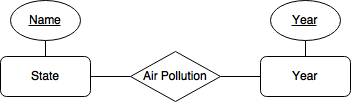
\includegraphics[width=\columnwidth]{cs458-ER-diagram-ass1}
 \caption{An ER diagram showing the relationship between our 3 tables: the State table has a primary key "name" and the Year table has a primary key "year", both of which are used to query on the Air Pollution table}
 \label{fig:ERdiagram}
\end{figure}


\begin{figure}
\centering
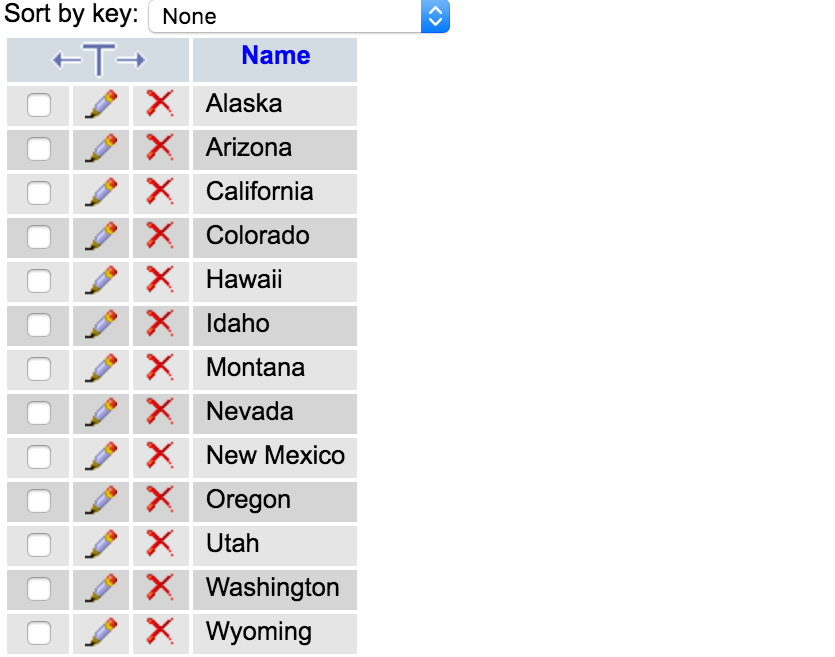
\includegraphics[width=\columnwidth]{state_db}
\caption{A visualization of the contents of the "state" table, with the "name" column serving as the primary key and key 
to index the "air pollution" table.}
\label{fig:stateDB}
\end{figure}

\begin{figure}
\centering
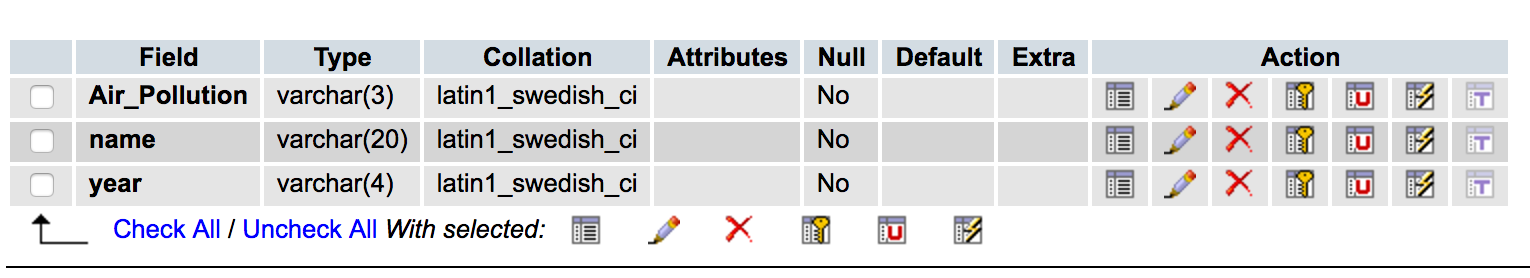
\includegraphics[width=\columnwidth]{air_poll_db}
\caption{The "air pollution" table's columns include "air pollution", "name", and "year" with "air pollution" 
containing all the values of the air pollution for each state and year, and "name" and "year" serving as keys.}
\label{fig:airPoll}
\end{figure}

\subsection{Design of the Interface}

We represent our data using an interactive tree map on a webpage. On the left hand side, users can select what year 
they want to view from 2007 to 2016, giving them the ability to see the changes in air pollution over the years. The 
size of the boxes on the tree map represent the magnitude of air pollution in a state in parts per million of harmful particulate matter. The larger the 
box, the higher the level of air pollution. The color of each box represents the change in air pollution levels from the previous 
year to the one selected. There will also be a scale above the treemap indicating what the range of the changes are for that year. 
A more negative number represents a higer decrease in harmful particulate levels - that is, a negative number means
that the state's air quality improved since the last measurement. On the other hand, a positive number represents an increase in harmful
particulate matter - and thus a decrease in air quality. The saturation of each box's color will serve as an indicator for the state's 
air quality. Our initial design for the visualization is represented in Figure \ref{fig:Design}.

\begin{figure}
\centering
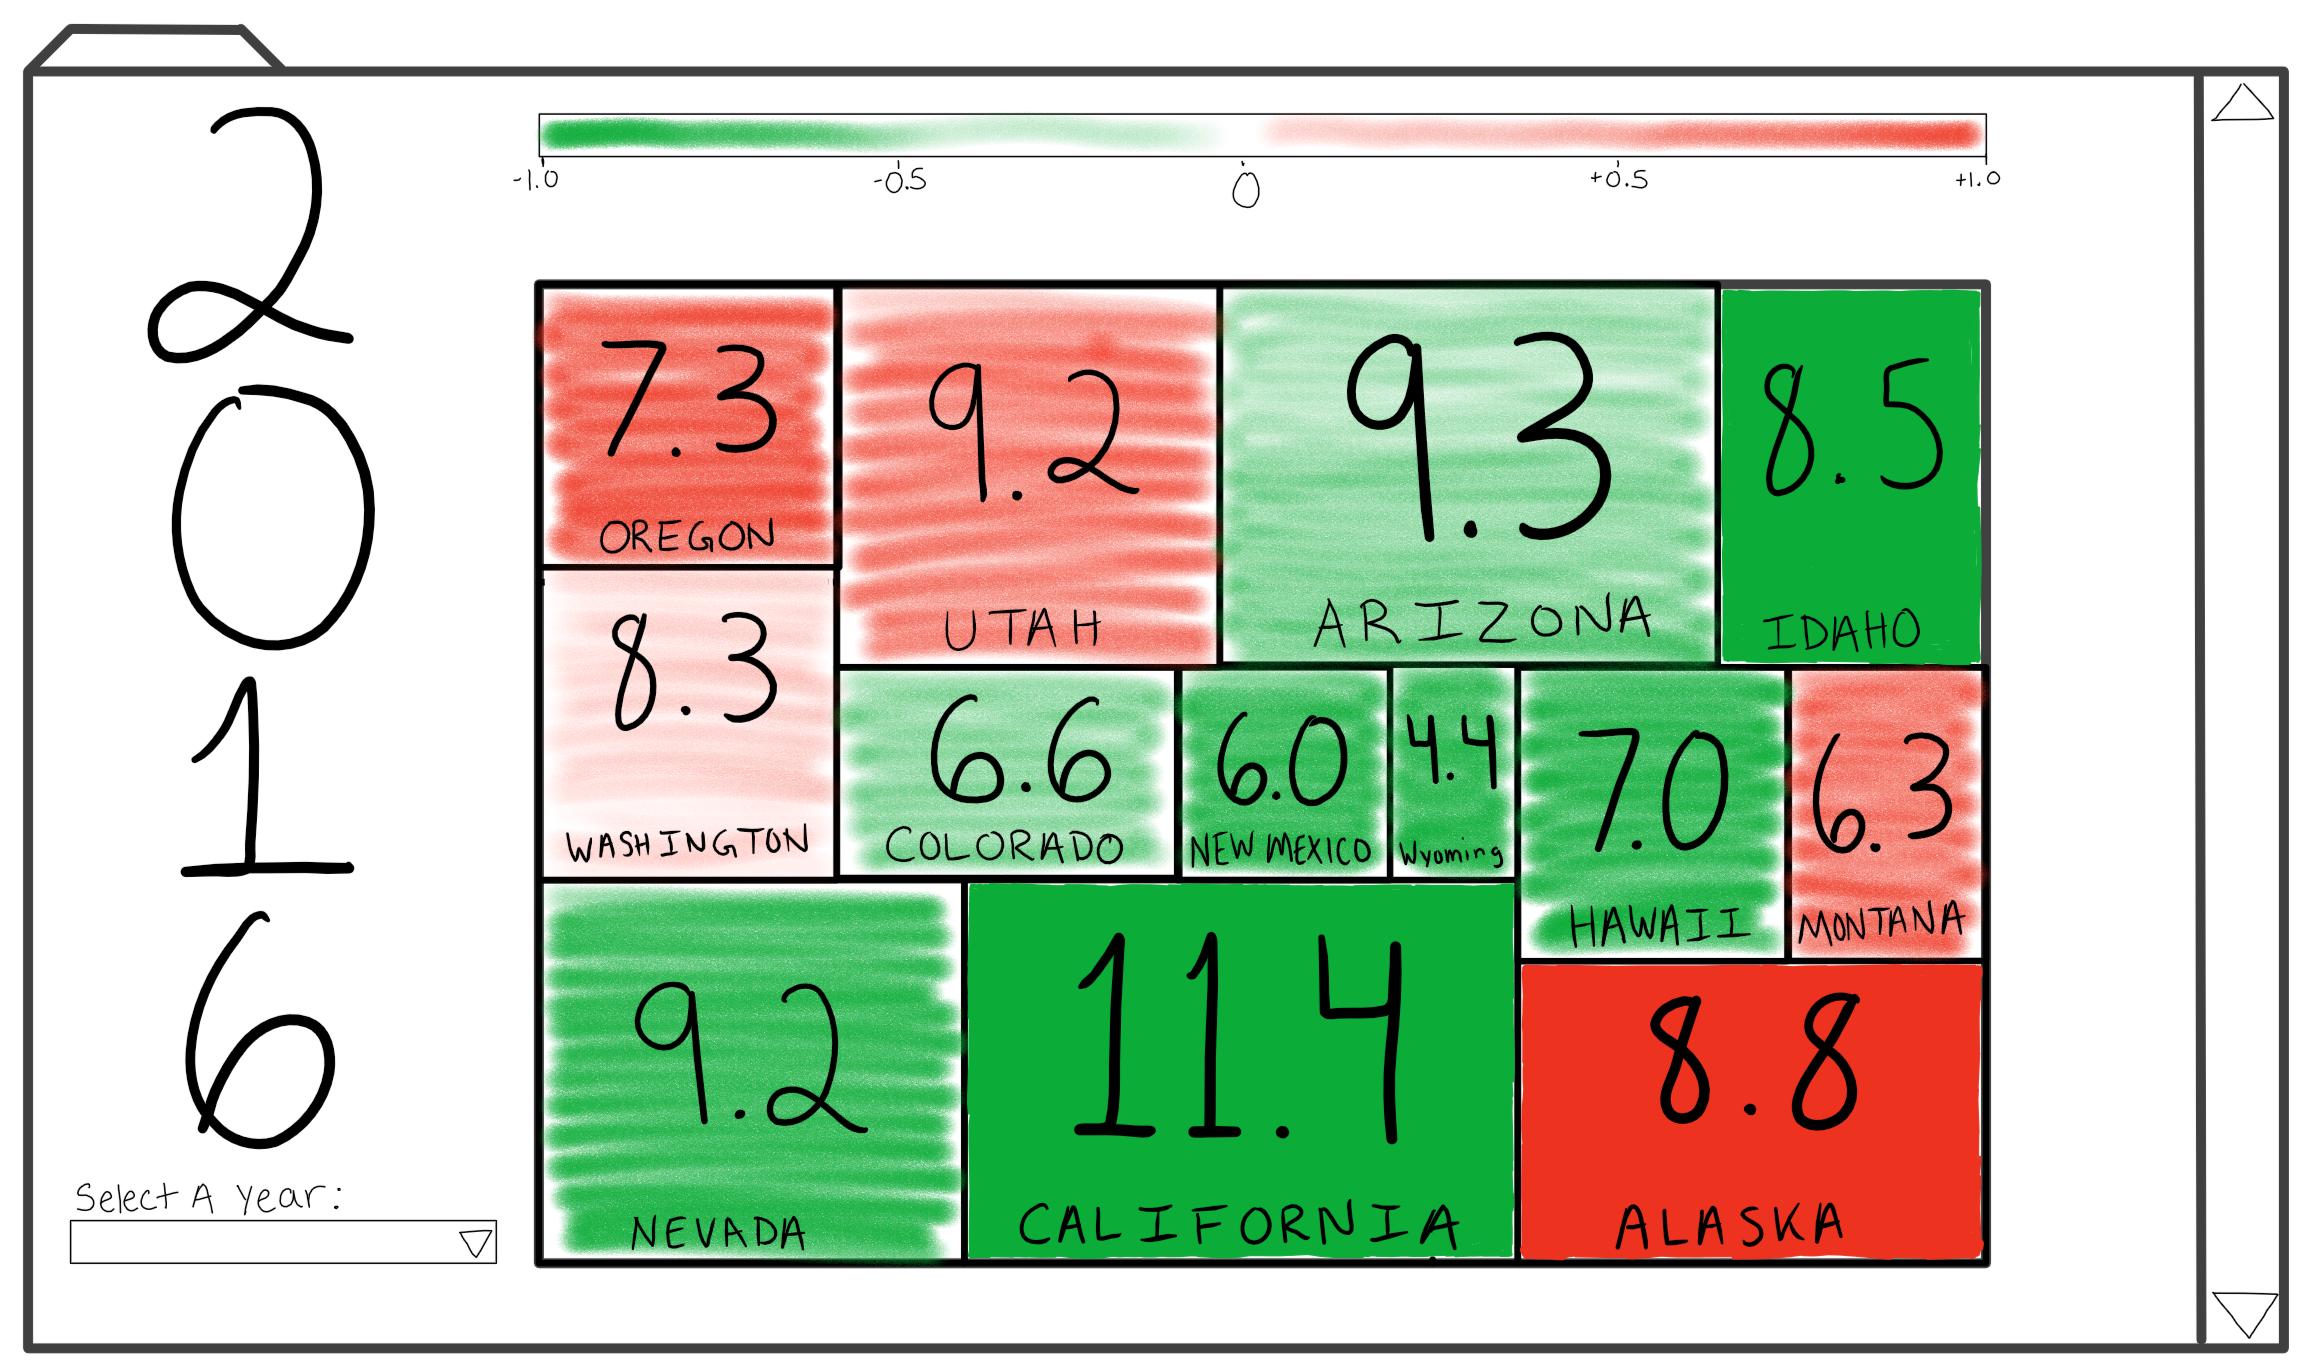
\includegraphics[width=\columnwidth]{HW1Design}
\caption{A visualization using a tree map describing the levels of air pollution in the western region by block size.}
\label{fig:Design}
\end{figure}

\subsection{Enhancement Over Existing Models}

After reviewing the current models available, our model provides an enhancement by providing an easy-to-understand
metaphor for non-experts to view how their state's air pollution is changing over time. We achieve this through size
and color changing to represent whether the air pollution levels are rising or lowering over time. For example, a large
orange** block means that a state's air pollution is rapidly increasing.

Previous models require an understanding of atmospheric sciences and are designed in mind for policy makers in the domain
of city planning[Zahran et al.]. While users with more experience in the domain of atmospheric sciences may use our
software, we hope to create a visualization that is accessible to users of all backgrounds.

\section{Implementation}

\subsection{Data Organization}
We created a relational database with 3 tables to store our data. The "state" table and "year" database are used to
index values stored within the "air pollution" database, as seen in the ER diagram in Figure \ref{fig:ERdiagram}.
We implemented the database on the ONID Database Server provided by Oregon State University. The contents
of the "state" diagram can be seen in Figure \ref{fig:stateDB} and the "air pollution" configuration can be found in 
Figure \ref{fig:airPoll}.

\subsection{Website}
Alannah

\subsection{Issues Encountered}
Alannah

\section{Results}
Alannah

\subsection{Insights}

** ??? I don't really know what kinds of insights we'd find but we will see I guess **

\subsection{Data Set}

** Yeah we already said this up in Methods so we could just reference that again I guess??? **

\subsection{Dimensions Used}

** Our visualization is both spatial (size of block) and temporal (can show change over time) so I guess talk about that/
why we chose that visualization/if it worked or not **

\subsection{Performance}

** no idea here since we're not running any sort of tests on it or doing any user studies lmao **

\subsection{Supplementary Materials}
** alannah said: link to source code - so I guess here we could link to our github or something **

\subsection{Domain Expert}

\section{Conclusion and Future Work}

Amb

\section{Acknowledgements}

Amb


\end{document}

